\section{Explaining V1 Receptive Field Formation}

\paragraph{Preprocessing}
Normalization and generation of input patches was done in a separate
preprocessing step. Preprocessing is called with
\begin{figure}[!htbl]
    \begin{verbatim}
$ python preprocess.py
\end{verbatim}
\end{figure}

Normalization step creates the file with suffix \texttt{\_normalized.data},
which contains a \texttt{numpy} array of normalized input image, serialized to
string. Afterwards, the file which describes patches is created. Its suffix is
\texttt{\_patches.data}. It contains $5000$ rows, where each row has the pixel
coordinates of upper-left corner of the $16\times16$ pixel patch. No two
patches are identical. This way of describing patches makes sure that additional
preprocessed data won't take too much memory, while still being easy to create
generated patches.

\begin{figure}[h]
\centering
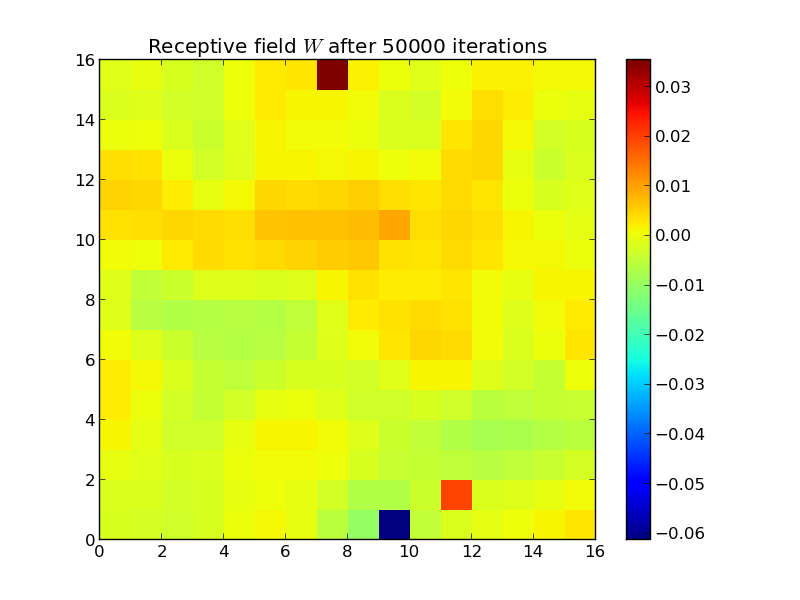
\includegraphics[width=0.7\textwidth]{../ex3/results1/img06}
\caption{}
\caption{Receptive field $W$ after $50000$ iterations}
\label{fig:img06}
\end{figure}

\begin{figure}[h]
\centering
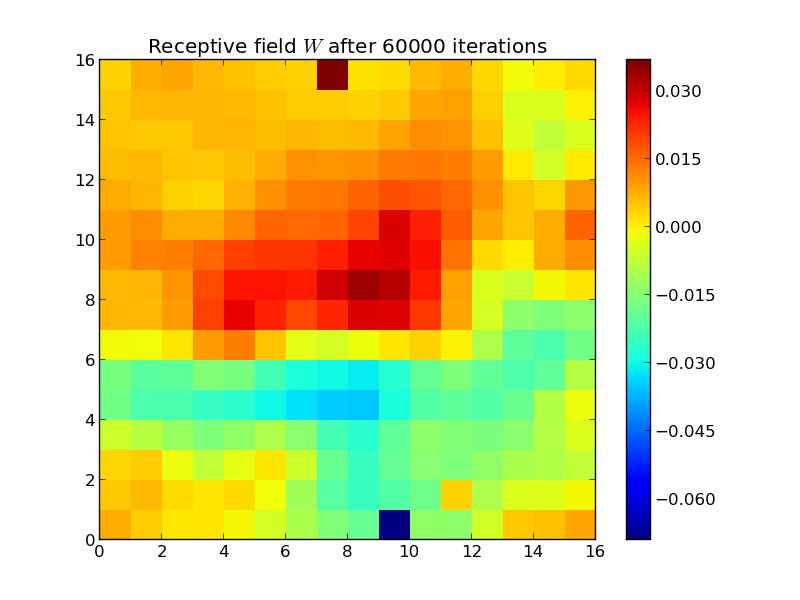
\includegraphics[width=0.7\textwidth]{../ex3/results1/img07}
\caption{Receptive field $W$ after $50000$ iterations. }
\label{fig:img07}
\end{figure}

\begin{figure}[h]
\centering
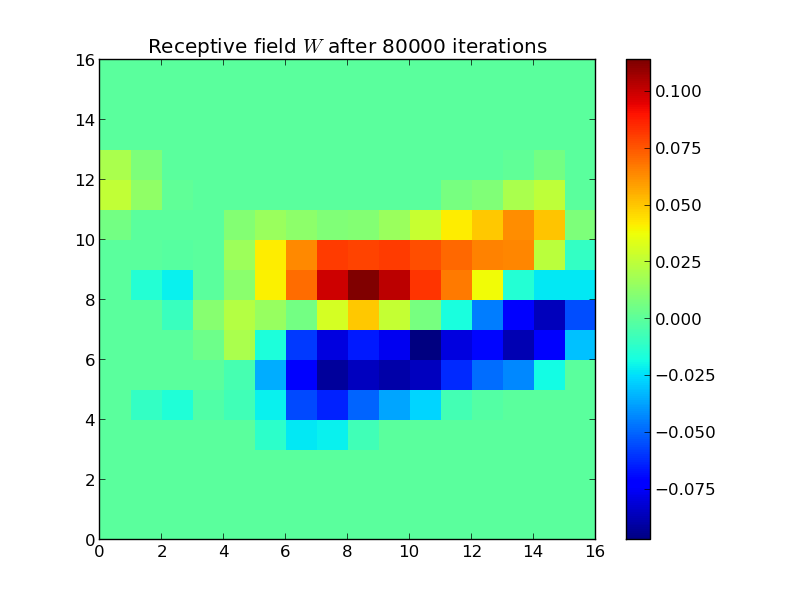
\includegraphics[width=0.7\textwidth]{../ex3/results1/img09}
\caption{}
\caption{Receptive field $W$ after $50000$ iterations}
\label{fig:img09}
\end{figure}

\begin{figure}[h]
\centering
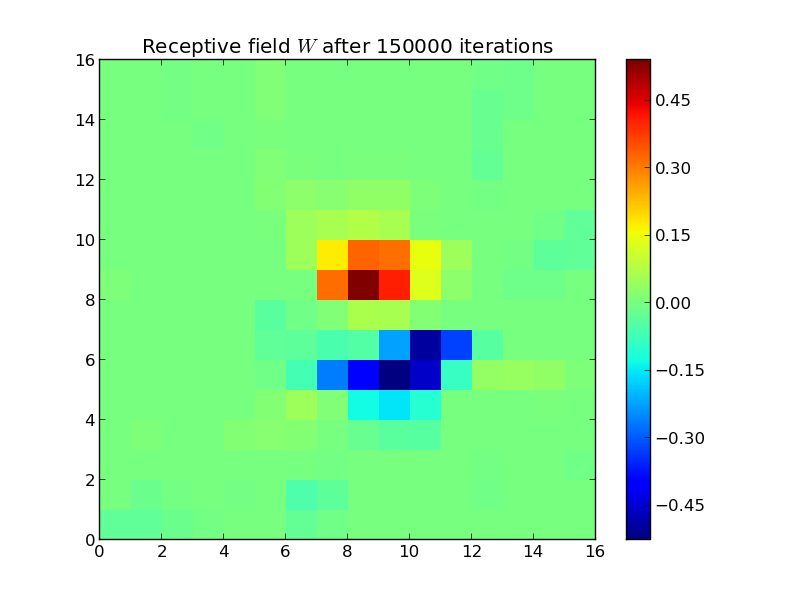
\includegraphics[width=0.7\textwidth]{../ex3/results1/img16}
\caption{}
\caption{Receptive field $W$ after $50000$ iterations}
\label{fig:img16}
\end{figure}

\begin{figure}[h]
\centering
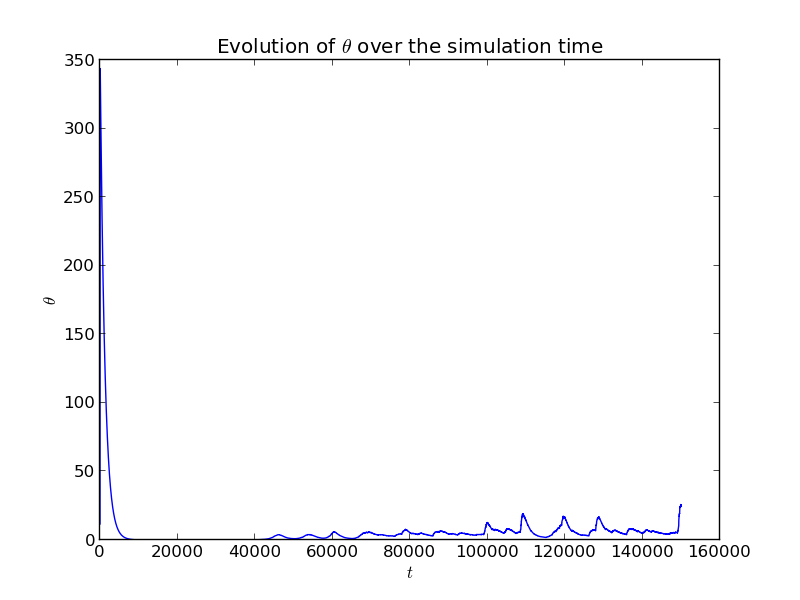
\includegraphics[width=0.7\textwidth]{../ex3/results1/theta}
\caption{}
\caption{Receptive field $W$ after $50000$ iterations}
\label{fig:theta}
\end{figure}

\paragraph{Simulation}
The simulation was done many times. Every simulation was done with $150000$
iterations, with $50000$ different patches. Every simulation has had different
permutations of patches, and occasionally, patches were constructed again using
preprocessing. Figures (mention them) show the typical development of a
receptive field. In the beginning--there is usually an initialization period, no
visible pattern. Then some lines start to emerge. In the end it is clearly
visible something similar to the Gabor filter. (need to comment this more
extensively)
